%!TEX root = ../phd-thesis-lei-ma.tex
%!TeX spellcheck = en-US
\chapter{Introduction}
\label{introduction}

\section{Properties of Neutrinos}

The neutrino has been one of the most astonishing particles in history. Its glorious history started with the observation of beta decay, i.e., the emission of electrons in nuclear decays, such as
\begin{equation*}
% {}^A_Z \mathrm X \to {}_{Z+1}^A\mathrm X + e^- +\bar \nu_e .
{}^{14}_{6} \mathrm C \to {}^{17}_{7}\mathrm N + \mathrm e^{-} + \bar\nu_{\mathrm e}.
\end{equation*}
The fact that the electron energy spectrum in the beta decay process is continuous indicates the existence of a third product other than ${}^{17}_{7}\mathrm N$ and $\mathrm e^-$. It was then proven to be an anti-neutrino. In the above reactions, the charged current weak interaction converts a down quark in the neutron to an up quark while releasing an electron and an anti-electron neutrino,
\begin{equation}
n\to p + e^- + \bar \nu_e .
\end{equation}
More generally, positron/electron emission and positron/electron capture processes are also neutrino-related nuclear reactions which are listed in Table~\ref{table:Neutrino_Reactions}. There are three different flavors of neutrinos, namely the electron flavor, the muon flavor, and the tau flavor as shown in Table~\ref{table:neutrino-properties}. The first direct detection of neutrinos was done by Clyde Cowan and Frederick Reines in 1956~\cite{Cowan1956} who used nuclear reactor neutrinos as the source of the experiment.

\begin{table}[ht]
\centering
 \begin{tabular}{|c | c | c|}
 \hline
 Reaction Type & Process & Mediator(s)   \\ [0.5ex]
 \hline
 Electron emission & ${}^A_Z X \to {}^A_{Z+1}X' + e^- +\bar \nu_e$ & $W^{\pm}$  \\
 Positron emission & ${}^A_Z X \to {}^A_{Z-1}X' + e^+ + \nu_e$ & $W^{\pm}$  \\
 Electron capture & ${}^A_Z X + e^- \to {}^A_{Z-1}X'  + \nu_e$ &  $W^{\pm}$ \\
 Positron capture & ${}^A_Z X + e^+ \to {}^A_{Z+1}X'  + \bar\nu_e$ &  $W^{\pm}$ \\
 [0.5ex]
 \hline

 $e^{\pm}$ annihilation &  $e^- + e^+  \to \nu + \bar\nu $  & $W^{\pm}$, $Z$ \\
%  Electron annihilation &  $e^- + e^+  \to \nu + \bar\nu $  & $Z$ \\
 Bremsstrahlung & $X+X' \to X + X' + \nu + \bar\nu$ & $Z$ \\
 [0.5ex]
 \hline

  $\nu (\bar\nu)$ capture & ${}^A_{Z}X + \overset{(-)}{\nu_e} \to {}^A_{Z\mp 1}X' + e^\pm $ & $W^{\pm}$\\
  [1ex]
 \hline
 $e^\pm\nu$ scattering & $e^- + \overset{(-)}{\nu_e} \to e^- + \overset{(-)}{\nu_e} $ &  $W^{\pm}$, $Z$ \\
 % $e^\pm\nu$ scattering & $e^{\pm} + \overset{(-)}{\nu_e} \to e^{\pm} + \overset{(-)}{\nu_e} $ &  $Z$ \\
 Nucleon scattering & $ {}^A_Z X + \overset{(-)}{\nu} \to {}^A_Z X + \overset{(-)}{\nu} $ &  Z\\
 [0.5ex]
 \hline
 \end{tabular}
 \caption{Neutrino related nuclear and leptonic reactions.}
\label{table:Neutrino_Reactions}
\end{table}

\begin{table}[ht]
\centering
 \begin{tabular}{|c | c | c|}
%  \hline
%  Property & Equation & Boson   \\ [0.5ex]
 \hline
  Electric Charge & 0\\
  \hline
  Spin & $1/2$ \\
\hline
 Mass & $<2~\mathrm{eV}$ \\
 \hline
 Interactions & Weak, Gravitation  \\
 \hline
 Flavors & $\nu_e$, $\nu_\mu$, $\nu_\tau$ \\
 \hline
 Chirality & Left \\
 \hline
 Hypercharge & $-1$ \\
 \hline

 \end{tabular}
 \caption{The physical properties of the neutrino~\cite{Patrignani:2016xqp}.}
\label{table:neutrino-properties}
\end{table}

\section{Stellar Neutrinos}


In addition to man-made sources, neutrinos are also produced by many astrophysical objects.% Astrophysical neutrino sources such as stars, AGN, Gamma-ray bursts, and supernovae reveal a great amount of information about these sources. Though neutrinos interact very weakly with matter and are hard to detect, it is important to theoretically inspect neutrino productions in astrophysical processes.
One of the such objects is the stellar core in which numerious nuclear reactions produce luminous neutrino fluxes.%In this section, the nuclear reactions in stars are reviewed as the background of neutrino oscillations in matter.
% \subsection{Nuclear Reactions in Sun and Solar Neutrino Flux}
The most important nuclear reactions in the Sun are the pp chain reactions. Fig.~\ref{fig:pp_Chain_Branching} shows the dominant energy sources of the Sun. In order to calculate the neutrino spectrum we need the neutrino production rate in each reaction and the branching ratios. Solar neutrinos are mostly produced in the pp reaction, Be electron capture and B decay which are labeled in red in Fig~\ref{fig:pp_Chain_Branching}:
\begin{align*}
&\mathrm{p+p\to {}^2H + e^+ +\nu_e}  & \mathrm{\leq 0.422MeV},\\
&\mathrm{{}^7Be + e^- \to {}^7Li + \nu_e} &\text{0.862MeV for 90\%},\\
&&\qquad \text{0.384MeV for 10\%}, \\
&\mathrm{{}^8B \to {}^8Be^* +e^+ +\nu_e}  & \mathrm{\leq 15 MeV}.
\end{align*}




\begin {figure*}%[!hbtp]
\centering
\begin{adjustbox}{width=\textwidth}
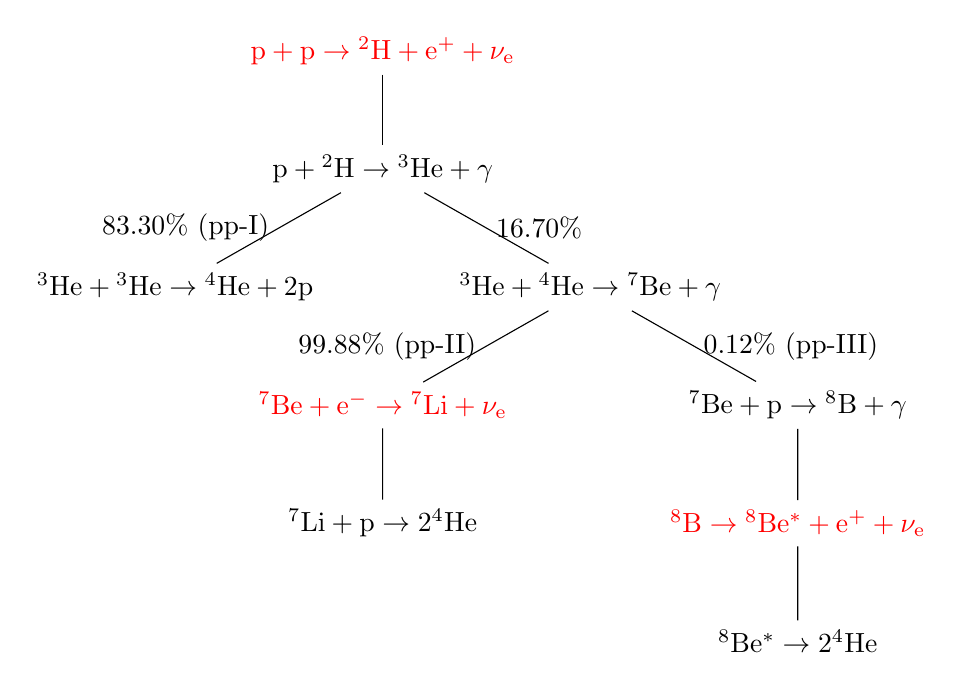
\begin{tikzpicture}[sibling distance=15em,
  every node/.style = {shape=rectangle,
    draw, align=center}
  edge from parent/.style = {draw, -latex},]]
  \node {\color{red}$\mathrm{p+p\to {}^2H + e^+ +\nu_e}$ }
    child { node {$\mathrm{p+{}^2H \to {}^3He + \gamma}$}
      child { node {$\mathrm{{}^3He+{}^3He \to {}^4 He + 2p }$}
          edge from parent node [left] {83.30\% (pp-I) } }
      child { node {$\mathrm{{}^3He+{}^4He \to {}^7 Be + \gamma }$}
        child { node {
\color{red}$\mathrm{{}^7Be + e^- \to {}^7Li + \nu_e}$
        }
        child { node { $\mathrm{{}^7Li + p \to 2{}^4He }$} }
        edge from parent node [left] {99.88\% (pp-II) } }
        child { node { $\mathrm{{}^7 Be + p \to {}^8 B + \gamma}$}
        child { node { \color{red}$\mathrm{{}^8B \to {}^8Be^* +e^+ +\nu_e}$ }
		child { node { $\mathrm{{}^8Be^* \to 2 {}^4He }$ } }}
        edge from parent node [right] {0.12\% (pp-III) } }
        edge from parent node [right] {16.70\%  } }};
\end{tikzpicture}
\end{adjustbox}
\caption{The pp chain reactions with the corresponding branching ratios. The branching ratios are taken from Ref.~\cite{Altmann2001}. }
\label{fig:pp_Chain_Branching}
\end{figure*}


% \begin{figure}[!hbtp]
% \centering
% 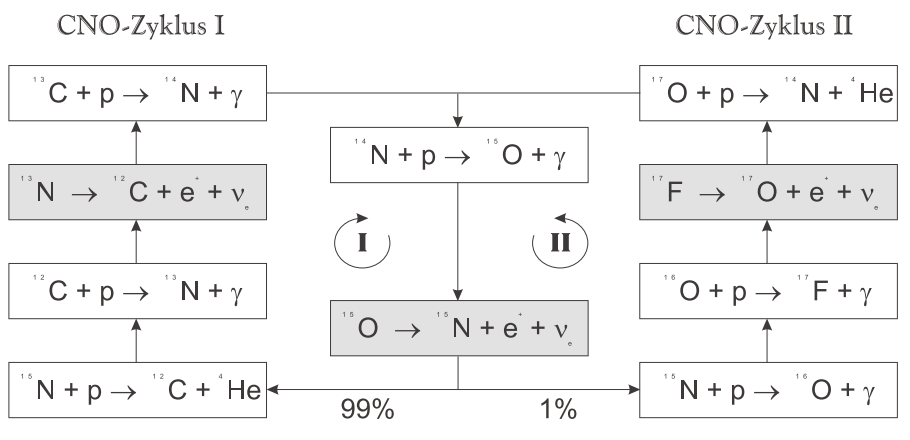
\includegraphics[width=\columnwidth]{chapters/assets/solar/cno_cycle.png}
% \caption{CNO cycle illustration~\cite{Adelberger2011a}.}
% \label{fig:cno_cycle}
% \end{figure}


Even without the knowledge of the detailed reactions, the conservation of the electric charge and the electron lepton number will lead to the overall neutrino production formula
\begin{equation}
\mathrm{4p+2e^- \to {}^4He + 2\nu_e }.
\end{equation}
It is important to notice that two neutrinos are emitted for each ${}^4He$ that is produced in the Sun. Using this simple relation, we can estimate the neutrino number flux emitted by the Sun. The energy released in each reaction is the difference between the initial and final rest masses of the particles,
\begin{equation}
Q=4m_p+2m_e-m_{{}^4 \mathrm{He}}=26.7\mathrm{MeV},
\end{equation}
where the mass of neutrinos are neglected. On average, each neutrino carries away an energy of $0.2\mathrm{MeV}$ and the rest of the energy is in the form of thermal energy $Q_\gamma=26.3\mathrm{MeV}$~\cite{Adelberger2011a}. %Energy flux density of solar photons near Earth is given by the solar constant $S_0$.
Since we know that each reaction produces 2 neutrinos while producing thermal energy $Q_\gamma$, the number flux of solar neutrinos near the Earth is roughly
\begin{equation}
\Phi_\nu = \frac{2 S_0}{Q_\gamma} \approx 6\times 10^{10} \mathrm{cm^{-2}s^{-1}},
\end{equation}
where the solar constant $S_0$ is the energy flux of solar photons on the top of the Eath atmosphere.
%Neutrinos are hard to detect but a large number flux makes it possible to detect solar neutrinos~\cite{Cleveland1998,Lande2003,McDonald2013}.

% On the other hand, the solar neutrinos have a certain energy spectrum due to the composition of nuclear reactions. Inside our Sun, two additional reactions other than pp neutrinos also produce neutrinos which are called pep and hep neutrinos.
% \begin{itemize}
% \item pep neutrinos are produced in
% \begin{equation}
% \mathrm{p + e^- + p \to {}^2H +\nu_e},
% \end{equation}
% which only has a branching ratio 0.4\% instead of the 99.6\% of pp reaction.
% \item hep neutrinos are produced in
% \begin{equation}
% \mathrm{ {}^3He + p \to {}^4He + e^+ \nu_e },
% \end{equation}
% which has a branching ratio of $2\times 10^{-5}\%$. As a comparison, the $\mathrm{{}^3He + {}^3He}$ has a branching ratio $85\%$ and $\mathrm{{}^3He + {}^4He}$ has a branching ratio $15\%$.
% \end{itemize}


As the detection of neutrinos becomes feasible, Ray Davis and John Bahcall et al worked out the solar neutrino flux and led the Homestake experiment to measure the solar neutrinos. The results revealed that the neutrino flux detected was less than what is predicted by solar models, which is the well-known solar neutrino problem~\cite{Bahcall1973}. It is known today that the solution to the problem is related to the neutrino. Electron neutrinos produced in the solar core transform to other flavors as they propagate, which is referred to as neutrino oscillations. The theory of neutrino oscillations was first proposed by Pontecorvo in 1968~\cite{Pontecorvo1968}. The field of neutrino oscillations has grown significantly into a broad field in physics since then.



\section{Supernova Neutrinos}



Another astronomical source of neutrinos is the core-collapse supernova explosion. Massive stars with a mass larger than 6−8 solar masses emit a huge amount of photons. However, violent delights have violent ends. When the core of a massive star run out of nuclear fuel, it collapses. During the collapse, the inner core is compressed to almost nuclear density, which has a stiff equation of state. The material falling onto the stiff core are bounced outward which forms a shock wave plowing through the inward flow leading to possible explosion. Those explosion forms the most power source of neutrinos as we know today~\cite{Raffelt1996wa}. On the other hand, supernova simulations show that the shock wave itself is not always energetic enough to produce the explosion~\cite{Janka2016b}. To revive the shock, more energy has to be deposited behind the shock. A possible solution is to introduce reheating of the shock by neutrinos~\cite{Janka2016b}. The energy of neutrinos emitted from a supernova explosion is about 10MeV scale~\cite{Janka2017}. The supernova explosion releases neutrinos with energy flux on the order of $10^{51}\mathrm{ergs\cdot s^{-1}}$~\ref{Bethe1985}. I can estimate the number density of neutrinos at the radius $R$ with energy $E$
\begin{equation*}
   n \sim  10^{18} \mathrm{cm^{-3}} \left(\frac{100\mathrm{km}}{R}\right)^2 \left(\frac{1\mathrm{MeV}}{E}\right),
\end{equation*}
which corresponds to the number flux
\begin{equation*}
  \Phi \sim 10^{27} \mathrm{cm^{-2} s^{-1}}\left(\frac{100\mathrm{km}}{R}\right)^2 \left(\frac{1\mathrm{MeV}}{E}\right).
\end{equation*}
Compared to the neutrino flux at the surface of the Sun, which is of the order $10^{15}\mathrm{cm^{-2} s^{-1}}$, supernova neutrinos is much denser. Neutrinos with such a high density would be a possible energy source to revive the shock. In order to implement neutrino-driven mechanism in computer simulations of supernovae, the flux and flavor content of neutrinos have to be known everywhere. Thus neutrino oscillations in dense matter become the a key to the supernova explosion problem. Observation-wise, neutrino signals are crucial for validation of our models for supernovae. In fact, detection of galactic core-collapse supernova neutrinos is on the task list of the Deep Underground Neutrino Experiment (DUNE)~\cite{Kemp2017}.




\section{Organization of the Disseration}


% As we have seen, it is crucial to understand neutrino flavors.
The rest of the disseration is organized as the follows.
In Chapter~\ref{chap:basics} I will review neutrino oscillations in vacuum and explain the flavor-isospin picture.
% Meanwhile, neutrino oscillations are ingredients of many other astrophysical, cosmological, and astronomical problems, such as neutron star mergers, dark matter, nucleosynthesis, etc. In order to gain a better understanding of neutrinos in these exotic environments, neutrino oscillations in dense matter background and dense neutrino background have to be thoroughly investigated. The seminal work by Mikheev--Smirnov--Wolfenstein proved neutrino interactions with matter background have significant effect on neutrino oscillations. They showed that neutrinos propagating through decreasing matter density experience a potential that alters the flavor conversions (MSW effect), which may also lead to maximum conversions between flavors~\cite{Mikheev:1986gs,wolf78,wolfensteinprd1979}. It is also know that neutrino oscillations in more general matter density profiles exhibit interesting phenomena. Resonances are found as the characteristic length scale in matter density profile and characteristic length scale of the neutrinos satisfies certain relations.
In chapter~\ref{chap:matter}, I will discuss in details neutrino oscillations in arbitrary matter density profiles, which is decomposed into Fourier modes and interpreted as a superposition of Rabi oscillations.
%Apart from dense matter background, neutrinos also interact with neutrinos themselves and introducing nonlinear dynamics. The neutrino self-interactions are analyzed using linear stability analysis.
In chapter~\ref{chap:dr}, I will review how neutrino self-interactions change neutrino oscillations when a significant neutrino backgroun is present such as core-collapse supernovae
%, as well as the dispersion relations in linear stability analysis. I will also discuss the neutrino halo problem. The halo problem exists because neutrino propagating out of dense matter medium will be scattered and forming a neutrino halo. Some of the neutrinos will propagate backward and interact with forward propagating neutrinos and alter the neutrino flavors. Mathematically speaking, the neutrino halo problem is a nonlocal boundary value problem. I will explain the numerical relaxation scheme that we developed, which we have proven to be a promising method to solve neutrino halo problem.
In chapter~\ref{chap:conclusion}, I will summarize my work and discusses the future explorations of the field.
